\documentclass[twocolumn,floatfix,aps,prd,nofootinbib]{revtex4-2}

\usepackage[utf8]{inputenc}
\usepackage[T1]{fontenc}
\usepackage{lmodern}
\input{glyphtounicode}
\pdfgentounicode=1
\usepackage{graphicx}
\usepackage{amssymb}
\usepackage{amsmath}
\usepackage{xcolor}
\usepackage{hyperref}
\usepackage{textcase}
\usepackage{placeins}
\usepackage[protrusion=true,expansion=false]{microtype}

\graphicspath{{figures/}}

\hypersetup{
    colorlinks=true,
    linkcolor=blue,
    filecolor=magenta,
    urlcolor=blue,
    citecolor=blue,
}
\urlstyle{same}
\emergencystretch=2em

\begin{document}

\title{\texorpdfstring{\MakeTextUppercase{The Bondi Dipole in Full Numerical Relativity: a Self-Accelerating Positive--Negative Mass Binary}}{The Bondi Dipole in Full Numerical Relativity: a Self-Accelerating Positive-Negative Mass Binary}}

\author{\MakeTextUppercase{Nikita M. Shirokov}}
\email{shirokov.nm@phystech.edu}
\affiliation{\textit{Independent Researcher, Moscow, Russia}}
\date{\today}

\begin{abstract}
Bondi observed in 1957 that bodies whose active gravitational masses have opposite signs should \emph{self-accelerate}: the negative one chases the positive one it repels, and the pair runs off together. Seven decades of analyses treated only point particles or exact metrics; here we present $3{+}1$ numerical-relativity evolutions of a ``Bondi dipole,'' built on what is, to our knowledge, the first stable, asymptotically flat star with negative total (ADM) mass dynamically evolved in numerical relativity---an object that proved the most robust in the campaign, its reversed gravity diluting rather than re-accreting its own shed field. Two complex scalar fields share identical dynamics; only the phantom sector sources Einstein's equations with a minus sign: inertial and passive masses positive, active mass negative. The measurements rest on twenty uniform-grid evolutions spanning three resolutions per configuration, $\Delta x = 0.50$, $0.33$ and $0.25$. Released at rest, the mixed pair---and only the mixed pair---self-accelerates as Bondi predicted: in the reference configuration, separation $d_0=12$ at $\Delta x=0.25$, the pair barycentre drifts $+1.64$ by $t=60$, $46$ times the two-canonical control and $142$ times the two-phantom one, while the drift itself is stable to $6.3\%$ across the resolution ladder and the controls converge away as the grid is refined. The drift reverses when the stars swap places (to $4.7\%$) and scales with the phantom's active mass to $0.7$--$3.9\%$ across the clean window, while the phantom's own fall is independent of its own mass to $0.4$--$2.6\%$. The geometry co-signs the kinematics: the $\ell=2$ Weyl-curvature amplitude rises in lockstep with the runaway speed (correlation $0.996$) and reproduces under mirror reflection to $4.7\%$; on a double-size box the four wave-zone shells $r=16$--$40$ agree on one outgoing wave to $1.1$--$1.4\times$ and the amplitude is box-independent to $0.2\%$. The conserved signed source closes the gravitational dipole-radiation channel at leading order, and in the signed bookkeeping the accelerating pair's sector momenta cancel to a residual $2.6$--$4.0\times$ smaller that matches the point-mass sum $M_+v_+ + M_-v_-$ to about $10\%$ over $20\le t\le30$---Forward's accounting carried over quantitatively to finite-size matter.
\end{abstract}

\maketitle

\section{Introduction}
\label{sec:intro}

Bondi~\cite{bondi1957} gave negative mass its modern treatment, distinguishing inertial, passive, and active gravitational mass and noting the striking consequence of mixing signs: a negative-mass body is \emph{attracted} by a positive one, the positive body is \emph{repelled} by the negative one, and the pair runs off together (Fig.~\ref{fig:schematic})---momentum conserved, because the negative body's contribution is negative. Bonnor and Swaminarayan~\cite{bonnor_swami1964} found exact solutions for uniformly accelerated opposite-mass pairs, later generalized in Ref.~\cite{bicak1983}; Bonnor~\cite{bonnor1989} asked why mass is positive and found no answer in the theory. Forward~\cite{forward1990} analyzed the Newtonian two-body problem exhaustively---for equal and unequal mass magnitudes alike---showing ``in tedious detail'' that the self-accelerating pair violates neither momentum nor energy conservation; objections to negative mass must be sought elsewhere~\cite{hoffmann1966,martins1980}.

\begin{figure}[t]
\centering
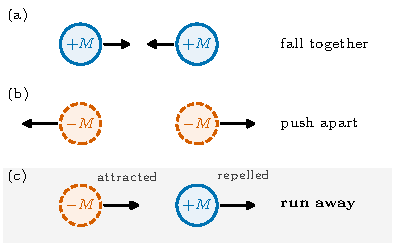
\includegraphics{fig_schematic.pdf}
\caption{Bondi's sign rules for two bodies released at rest, in the style of Forward's analysis~\cite{forward1990}. Every body here has positive inertial and passive mass; only the \emph{active} (source) mass carries a sign---negative for the dashed bodies. (a)~Two positive-mass stars attract each other and fall together; (b)~two negative-mass stars repel each other and push apart. In both cases the forces oppose, and the pair barycentre stays put. (c)~The mixed pair---the Bondi dipole: the positive star is repelled by the negative one, the negative star is attracted by the positive one, so both forces point the \emph{same} way and the pair barycentre accelerates, the system carrying zero total momentum in the signed bookkeeping. Each row is realized as a run of the matrix in Table~\ref{tab:matrix}, and the pair barycentre named in each row is the quantity every later figure measures.}
\label{fig:schematic}
\end{figure}

Why does this deserve a full numerical-relativity campaign? Because nothing in Einstein's equations forces mass to be positive---positivity is a theorem only once energy conditions are imposed on the matter: for asymptotically flat data obeying the dominant energy condition the ADM mass is provably nonnegative~\cite{schoen_yau1979,witten1981}, so an asymptotically flat negative-mass body \emph{must} violate an energy condition (with de Sitter asymptotics, remarkably, it need not~\cite{mbarek2014}, and Mann~\cite{mann1997} showed that regions of negative energy density can collapse to black holes whose exterior spacetimes carry negative mass and non-trivial topology)---and modern physics keeps producing sources that strain those conditions: Casimir energies, quantum fields in curved spacetime, a dark-energy sector whose observational fits tolerate phantom equations of state~\cite{caldwell2002}. Every traversable wormhole~\cite{morris_thorne1988} and warp spacetime~\cite{alcubierre1994} requires matter of exactly this kind, and the standing objection to all of them is Bondi's runaway itself: matter that accelerates for free looks like a perpetual-motion machine, hence absurd~\cite{hoffmann1966,martins1980}. That objection has only ever been examined for point particles and special exact metrics. Whether the runaway actually happens in full nonlinear general relativity---with finite bodies, backreaction, and radiation---and whether momentum conservation really survives it, is a concrete, checkable question. Answering it also requires learning to evolve energy-condition-violating matter stably in numerical relativity at all, a capability any quantitative study of exotic spacetimes will need.

All of the analyses above, seven decades of them, treat point particles, prescribed metrics, or frozen mass parameters. The nonlinear evolutions that do exist for energy-condition-violating matter---ghost-scalar wormhole spacetimes, in spherical symmetry~\cite{shinkai2002,gonzalez2009}---concern single objects, and the phantom-field compact stars of Ref.~\cite{dzhunushaliev2014} are static constructions. None of these can say whether such a configuration can be posed as a \emph{consistent initial-value problem}---constraint-satisfying initial data for dynamical matter---or whether the runaway survives full nonlinear evolution with backreaction, radiation, and finite body size. That is the gap this paper closes; we are not aware of any previous $3{+}1$ evolution of a gravitationally bound positive--negative active-mass pair with dynamical, constraint-solved matter.

The question has acquired observational stakes while this work was being completed. Trivedi and Loeb~\cite{trivedi_loeb2026} proposed negative-mass binaries as sources of anomalous gravitational-wave signatures---anti-chirps, dispersal, and runaway motion---turning Bondi's paradox into an exclusion channel for real detectors. Nojiri and Odintsov~\cite{nojiri2026} argued from the opposite direction that negative-mass objects need not be exotic at all, arising as solutions of standard gravitational equations for a compact positive mass immersed in a cosmological fluid with negative cosmological constant, and constructed two-scalar and Einstein--Gauss--Bonnet models that support them; notably, they find that a bound positive--negative system \emph{can} form in that setting despite the repulsion. Our asymptotically flat, isolated pair is the complementary case, and it does not bind---it runs away.

Our contributions:
\begin{itemize}
    \item[(i)] A minimal field-theoretic realization of Bondi's sign structure: a \emph{bicomplex} scalar model in which both sectors obey identical Klein--Gordon dynamics and only the Einstein source is signed (Sec.~\ref{sec:model}).
    \item[(ii)] Dressed soliton stars for both signs, solved at fixed frequency as constraint-satisfying initial data---including, as far as we know, the first asymptotically flat star with negative total (ADM) mass dynamically evolved this way (Sec.~\ref{sec:initialdata}); static phantom-field stars~\cite{dzhunushaliev2014} and de Sitter negative-mass bubbles~\cite{mbarek2014} were known.
    \item[(iii)] A falsifiable run matrix---mixed pair at three separations, same-sector pairs, single stars, a mirrored pair, an equal-$|M|$ variant---run under identical numerics and, for every uniform-grid cell, at three resolutions (Sec.~\ref{sec:setup}).
    \item[(iv)] The result: the mixed pair, and only the mixed pair, self-accelerates, with a drift that is stable under grid refinement while the controls' residuals converge away (Sec.~\ref{sec:convergence}); the effect scales with the source mass, and its excess over the matched point-mass prediction falls with separation (Sec.~\ref{sec:results}).
    \item[(v)] The geometric witness: the $\ell=2$ Weyl amplitude rises in lockstep with the runaway speed and reproduces under mirror reflection, and a double-size box places four extraction shells on one outgoing wave (Sec.~\ref{sec:weyl}).
    \item[(vi)] An honest accounting of the diagnostic biases that can mimic or mask the physics under test, with their measured scope (Sec.~\ref{sec:caveats}).
\end{itemize}

One more first rode along with the physics: every evolution here ran on a single GPU, with \texttt{GRTeclyn}~\cite{grteclyn}, the AMReX-based~\cite{amrex} GPU port of \texttt{GRChombo}~\cite{grchombo}. Together with the ghost-scalar wormhole collapse campaign of Ref.~\cite{shirokov2026}, run with the same code, these are to our knowledge the first evolutions of energy-condition-violating matter in GPU-native numerical relativity, and the fact that the whole campaign---initial data, twenty uniform-grid production runs, and their diagnostics---fit on one multi-GPU node is itself a statement about how accessible this class of question has become.

Throughout, $G=c=1$ and the scalar mass sets the unit, $m=1$. Drifts along the pair axis are quoted as $\Delta x = x(t)-x(0)$, and $d$ denotes the instantaneous barycentre separation. The paper follows the build order: Sec.~\ref{sec:model} defines the matter model, Sec.~\ref{sec:initialdata} constructs the stars and the initial data, Sec.~\ref{sec:setup} lays out the campaign, Sec.~\ref{sec:results} the measurements, Sec.~\ref{sec:weyl} the gravitational-wave signature, and Secs.~\ref{sec:caveats}--\ref{sec:discussion} their limits and meaning.

\section{The bicomplex scalar model}
\label{sec:model}

We first need matter that can realize Bondi's sign structure while remaining an honest field theory, and the requirements are stiffer than they look. The bodies must keep canonical \emph{dynamics}---positive inertial and passive mass---while only their gravitational \emph{source} changes sign; they must form stable, localized stars; and the negative-mass star must be held together by something other than gravity, because its own gravity pushes it apart---the self-repulsion of negative-mass material that Forward's analysis already identified~\cite{forward1990}. Each obvious alternative fails one of these tests. The negative-mass Schwarzschild spacetime cannot be evolved as a puncture: it is a naked singularity---no horizon to excise behind---and Gleiser and Dotti~\cite{gleiser2006} exhibited exact, everywhere-smooth solutions of its linearized Einstein equations that grow exponentially, so a $3{+}1$ evolution would amplify them from truncation error alone; nor does the spacetime contain any matter from which to build constraint-satisfying initial data. A negative-energy fluid has no equilibrium to sit in: a fluid star is bound by the very attraction being flipped, and Bonnor's static negative-mass spheres~\cite{bonnor1989} demand an inverted interior---negative rest density against positive pressure, random motions exerting tension rather than pressure---with no non-gravitational force to restore the configuration once perturbed. A ghost scalar---kinetic term reversed in the Lagrangian---does source gravity negatively, but its field dynamics reverse too, so its inertial and passive masses flip along with the active one (Forward's all-negative matter~\cite{forward1990}, not the active-only signature under test), and such fields, evolved in numerical relativity as wormhole support, either collapse or explode~\cite{shinkai2002,gonzalez2009}; in our own companion evolutions of the ghost-supported Ellis--Bronnikov wormhole, truncation-level noise alone sufficed to trigger the explosive branch, with a measured e-folding time of $0.11\,M$~\cite{shirokov2026}.

What passes is a \emph{soliton}: matter self-bound by its own interactions, for which gravity is a dressing rather than the binding agent. We therefore take two independent complex scalar fields, $\Phi_+$ (\emph{canonical}) and $\Phi_-$ (\emph{phantom}), living on one spacetime. Both are governed by the same potential, the standard sextic form of Q-ball and solitonic boson-star studies~\cite{friedberg1976,coleman1985,friedberg1987},
\begin{equation}
V(|\Phi|^2)=\tfrac12 m^2|\Phi|^2-\tfrac14\lambda|\Phi|^4+\tfrac16\mu|\Phi|^6 ,
\label{eq:potential}
\end{equation}
where $m$ is the field mass and $\lambda,\mu>0$ are self-coupling constants. Each term has a fixed job: the mass term makes the field oscillate, the attractive quartic ($-\lambda$) lets the field clump into localized, self-bound lumps, and the repulsive sextic ($+\mu$) stops the clumping short of collapse---with the quartic alone, which is critical in three dimensions, a lump either collapses or disperses. With all three terms the flat-space theory supports Q-ball--type solitons. (``Lump'' is our generic word for such a self-bound blob of field; it becomes a ``star'' once gravity dresses it.) Self-binding is what lets the phantom star exist at all: a gravity-bound body cannot survive having its gravity reversed, but a field-bound lump merely gets dressed---compressed by attractive gravity in one sector, dilated by repulsive gravity in the other (Sec.~\ref{sec:initialdata}). Sharing one potential is deliberate, not economy: it makes the matter physics of the two sectors \emph{identical}, so that the single sign introduced next is the only difference between them---and therefore the only possible cause of any asymmetry the simulations show.

The entire sign structure lives in one place: the Einstein equations are sourced by the \emph{signed} sum of two canonical stress tensors,
\begin{equation}
G_{\mu\nu}=8\pi\left(T_{\mu\nu}[\Phi_+]-T_{\mu\nu}[\Phi_-]\right),
\label{eq:einstein}
\end{equation}
while the field equations of \emph{both} sectors keep their canonical form,
\begin{equation}
\Box\,\Phi_\pm=2\,\frac{\partial V}{\partial|\Phi|^2}\,\Phi_\pm ,
\label{eq:kg}
\end{equation}
the factor of $2$ fixed by the $\tfrac12$-normalized kinetic term of the sector Lagrangian below. In the $3{+}1$ language the matter sources seen by normal observers---the energy density $\rho$ and momentum density $S_i$ that feed the ADM constraint and evolution equations---are accumulated per sector with a sign $\epsilon_\pm=\pm1$:
\begin{equation}
\rho=\sum_{s=\pm}\epsilon_s\,\rho[\Phi_s],\qquad
S_i=\sum_{s=\pm}\epsilon_s\,S_i[\Phi_s],
\label{eq:adm_sources}
\end{equation}
and likewise for $S_{ij}$, each bracket being the standard scalar-field expression.

Three consistency statements follow from the structure, and are worth making explicit. The model derives from the action
\begin{equation}
S=\int d^4x\,\sqrt{-g}\left[\frac{R}{16\pi}+\mathcal{L}[\Phi_+]-\mathcal{L}[\Phi_-]\right],
\label{eq:action}
\end{equation}
with the canonical $\mathcal{L}[\Phi]=-\tfrac12\nabla_\mu\Phi^*\nabla^\mu\Phi-V(|\Phi|^2)$: the overall sign of a sector's Lagrangian cancels from its Euler--Lagrange equations---hence the canonical dynamics of Eq.~\eqref{eq:kg}---but survives the metric variation---hence the signed source of Eq.~\eqref{eq:einstein}. Bianchi consistency is then automatic: each sector's stress tensor is separately conserved on shell, so the signed sum sourcing $G_{\mu\nu}$ is conserved too. And well-posedness is inherited: the principal part of CCZ4 plus two canonical Klein--Gordon fields is exactly that of the standard system---the sector sign enters only algebraic source terms---so strong hyperbolicity is unaffected. What is \emph{not} claimed is quantum viability: a sector entering gravity with negative energy admits graviton-mediated vacuum decay into positive--negative pairs~\cite{carroll2003,cline2004}; the model is a classical probe, in the sense of the remarks below.

This structure delivers exactly the mass signature Bondi's argument needs. How the phantom \emph{moves} is set by its field equation~\eqref{eq:kg}, which is completely ordinary: the phantom field resists acceleration and falls toward gravitational wells like any other matter---in Bondi's vocabulary, its \emph{inertial} and \emph{passive} masses are positive. How the phantom \emph{gravitates} is set by the minus sign in Eq.~\eqref{eq:einstein}: the field it sources is that of a negative mass, so its \emph{active} mass is negative and it repels everything. In particular its Arnowitt--Deser--Misner (ADM) mass---the total mass a distant observer would infer from the far gravitational field---comes out negative.

Now place one star of each kind side by side. The canonical star attracts the phantom, which falls toward it; the phantom repels the canonical star, which retreats. Both accelerations point the same way, from phantom toward canonical, and the pair runs off together. This is the precise sense in which ``Newton's third law fails'' here: the two forces point in the \emph{same} direction rather than opposing each other. No conservation law breaks. The conserved momentum belongs to the total signed stress-energy of Eq.~\eqref{eq:adm_sources}, in which the phantom's momentum enters with a minus sign; the two growing momenta cancel, and the accelerating pair carries near-zero total momentum---the cancellation Forward exhibited for the Newtonian problem~\cite{forward1990}, here general-relativistic.

Two honest remarks. The phantom sector violates the null energy condition by construction; this is a model of \emph{if such matter existed, what would gravity do}, in the spirit of phantom cosmology~\cite{caldwell2002}, not a claim that it exists. And our sign structure differs from Forward's all-four-masses-negative matter~\cite{forward1990}: here only the source sign flips. The two-body phenomenology is the same, because passive and inertial mass cancel---each body's acceleration is set by the \emph{other} body's active mass, the property under test.

The model is implemented in \texttt{GRTeclyn}~\cite{grteclyn,grchombo,amrex}, evolving CCZ4~\cite{alic2012} plus the two complex fields, with Eq.~\eqref{eq:adm_sources} accumulated star by star in the initial-data solver \texttt{GRTresna}~\cite{grtresna} so that one constraint solve can carry mixed-sign matter.

\section{Initial data: gravitationally dressed solitons}
\label{sec:initialdata}

The task of this section is to turn the model into two stars on one initial slice: fix the couplings, solve each star as a spherical equilibrium, transfer the solved profiles onto the evolution grid, and solve the constraints for the pair. None of these steps is optional---the potential alone, without the gravitational dressing and the exact seeding below, produces no star that survives evolution.

\subsection{Couplings}

The potential~\eqref{eq:potential} has three parameters: the mass $m=1$ (our unit) and the self-couplings $\lambda,\mu$. One more number needs a name before they can be chosen. A soliton of this theory oscillates coherently, $\Phi\propto e^{-i\omega t}$, and the frequency $\omega$ labels the solution family: $\omega=m$ is the free-field limit, the deficit $1-\omega$ is the binding energy per unit mass, and lower $\omega$ means a more tightly bound, more massive lump.

Two combinations of the couplings control the physics. The dimensionless ratio $\lambda^2/\mu$ sets the \emph{shape} of the potential and, through it, the lowest frequency a flat-space soliton can have: the classic Q-ball existence bound $\omega_{\min}^2=\min_{|\Phi|}\bigl[2V/|\Phi|^2\bigr]$~\cite{coleman1985} evaluates, for the potential~\eqref{eq:potential}, to $\omega_{\min}=\sqrt{1-3\lambda^2/16\mu}$, attained at the field value $\sqrt{3\lambda/4\mu}$---which is also the interior (``thin-wall'') amplitude of a large soliton. All runs use $\lambda^2/\mu=4.8$, so $\omega_{\min}=0.316$ and the working frequency $\omega=0.55$ sits comfortably inside the allowed range, at $45\%$ binding. With the shape fixed, the remaining freedom---the overall strength of the couplings---sets that amplitude, and with it how strongly the lump gravitates: scaling $\lambda$ and $\mu$ up together at fixed $\lambda^2/\mu$ makes the field fainter and its self-gravity weaker. The values used everywhere, $\lambda=10240$ and $\mu\simeq2.18\times10^{7}$ (amplitude ${\simeq}0.019$), are not a free choice: every more strongly gravitating combination produced stars that collapsed or dispersed, and these couplings are the first at which a dressed $\omega=0.55$ star exists at all.

\subsection{The dressed-star problem}

The problem, stated plainly: a flat-space soliton solves the field equation with gravity switched off, and such an object cannot simply be placed on an initial slice. It fails as initial data, because the Hamiltonian and momentum constraints know about the field's energy and are violated by a bare Q-ball; and it fails as an equilibrium, because once its own gravity acts the profile is no longer an eigenstate---seeded anyway, the star breathes, sheds, and disperses. The star we need is solved with its gravity \emph{on}: field and metric adjusted together until the profile is the eigenstate of the very spacetime it curves. That is what ``dressed'' means here.

Dressing the soliton in its own gravity is the boson-star problem~\cite{kaup1968,ruffini1969} with a sextic self-interaction (see Ref.~\cite{liebling2023} for a review), posed for both source signs. Inserting the harmonic ansatz $\Phi=\varphi_0(r)\,e^{-i\omega t}$ and a conformally flat, maximally sliced metric $ds^2=-\alpha^2dt^2+\psi^4\delta_{ij}dx^idx^j$ into Eqs.~\eqref{eq:einstein}--\eqref{eq:kg} reduces the problem to three coupled ordinary differential equations in $r$ (the standard boson-star reduction~\cite{liebling2023}),
\begin{align}
\psi''+\tfrac{2}{r}\psi' &= -2\pi\psi^5\rho, \nonumber\\
\alpha''+\left(\tfrac{2}{r}+\tfrac{2\psi'}{\psi}\right)\alpha' &= 4\pi\psi^4\alpha\,(\rho+S), \label{eq:starode}\\
\varphi_0''+\left(\tfrac{2}{r}+\tfrac{\alpha'}{\alpha}+\tfrac{2\psi'}{\psi}\right)\varphi_0' &= \psi^4\!\left(\frac{dV}{d\varphi_0}-\frac{\omega^2}{\alpha^2}\varphi_0\right), \nonumber
\end{align}
with $\rho=\tfrac12\omega^2\varphi_0^2/\alpha^2+\tfrac12\psi^{-4}\varphi_0'^2+V$ and $\rho+S=2\omega^2\varphi_0^2/\alpha^2-2V$; here $dV/d\varphi_0\equiv2\varphi_0\,\partial V/\partial|\Phi|^2$ is the derivative of the effective real-field potential $V(\varphi_0^2)$, the factor of $2$ matching Eq.~\eqref{eq:kg}. \textbf{The phantom star is obtained by flipping the sign of $\rho$ and $\rho+S$ in the metric equations only}; the Klein--Gordon line keeps its canonical form, mirroring Eqs.~\eqref{eq:einstein}--\eqref{eq:kg}. The result is a self-interaction-bound soliton with repulsive gravity: $\psi<1$, $\alpha>1$ in the core (reversed for the canonical star) and negative ADM mass.

We integrate Eqs.~\eqref{eq:starode} by shooting; the solver and the $M(\omega)$ family scan behind Fig.~\ref{fig:family} ship in the results pack. Solving at \emph{fixed frequency} matters: heavy-branch sextic stars sit a fraction of a percent below the effective-potential top, so at fixed central amplitude the eigenvalue in $\omega$ is an exponentially thin needle, and a shooter on $\omega$ lands on the light branch (a request for the $\omega=0.55$ star returned a $5\times$ lighter $\omega=0.75$ star). Instead we bisect the central amplitude $\varphi_c$ at fixed integration-frame frequency and outer-iterate until the rescaled frequency $\omega/\alpha_\infty$ matches the request, to ${\sim}10^{-5}$.

\begin{figure}[t]
\centering
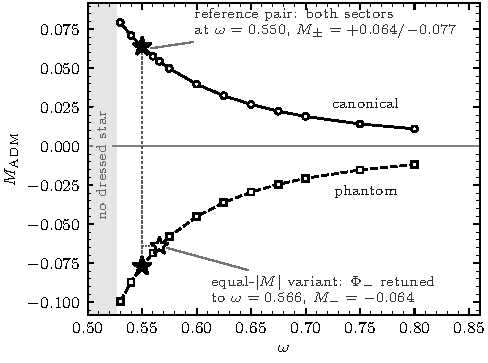
\includegraphics{fig_family.pdf}
\caption{ADM masses of the spherical stars against the field oscillation frequency $\omega$, from Eqs.~\eqref{eq:starode} at the working couplings: the canonical branch ($M_{\rm ADM}>0$) and the phantom branch ($M_{\rm ADM}<0$). Lower frequency means deeper binding and larger $|M_{\rm ADM}|$; in the shaded region the solver finds no gravitationally dressed star. At equal frequency the phantom star is the heavier in magnitude ($20.3\%$ at $\omega=0.550$, $4.3\%$ at $\omega=0.80$), its repulsive self-gravity spreading it over more volume. Filled stars, joined by the dashed line: the reference pair, both sectors at $\omega=0.550$. Open star: the equal-$|M_{\rm ADM}|$ variant, whose phantom is retuned to $\omega=0.56598$ so that $M_-=-0.063950$ matches the canonical star to one part in $10^5$.}
\label{fig:family}
\end{figure}

Figure~\ref{fig:family} shows both families. The reference pair uses the two $\omega=0.550$ stars: canonical ($\varphi_c=0.019695$, $M_{\rm ADM}=+0.063951$, central lapse $0.9773$) and phantom ($\varphi_c=0.019589$, $M_{\rm ADM}=-0.076962$, central lapse $1.0249$). Because both are taken at the \emph{same} frequency, and the phantom branch is the heavier there, the reference pair is intrinsically unequal: $|M_-|/M_+=1.203$. For the equal-$|M|$ run of Sec.~\ref{sec:setup} the phantom is instead solved at $\omega=0.56598$, where $M_{\rm ADM}=-0.063950$ matches the canonical star's mass to one part in $10^5$. Matching the \emph{ADM} masses---rather than bare field amplitudes or Noether charges---is the choice Bondi's point-mass limit dictates: each body's exterior field, and hence the force it exerts on its partner, is set by its ADM mass alone. The different internal frequency this requires ($0.56598$ against $0.550$) is part of the phantom's equilibrium at that mass, not an extra knob.

\subsection{From radial profiles to three-dimensional initial data}

The solved profiles $\varphi_0(r)$, $\alpha(r)$, $\psi(r)$ are next transferred onto the Cartesian evolution grid, one star at each release position. Two details of this step are essential. First, the seeded amplitude must be the star's own solved $\varphi_c$---any rescaling de-tunes the eigenstate. Second, a boson star is stationary but not static: its phase rotates, so the field carries a $U(1)$ momentum, and the momentum conjugate to $\Phi$ is defined per unit \emph{proper} time of the normal observers, $\Pi=\alpha^{-1}\partial_t\Phi$ for zero shift. The harmonic phase therefore seeds
\begin{equation}
\Pi_{\rm im}=-\frac{\omega}{\alpha(r)}\,\varphi_0(r);
\label{eq:pi_im}
\end{equation}
a flat-space seed ($\alpha\equiv1$) would start the star slightly off its eigenstate everywhere the lapse differs from one, which is why the star tables carry $\alpha(r)$. Each star is seeded from its own table with its own frequency; giving the $\omega=0.56598$ star a global $\omega=0.550$ phase velocity would likewise de-tune it.

\texttt{GRTresna} then solves the constraints for the pair (CTTKHybrid scheme~\cite{cttk}, sources summed with their signs star by star) to $0.1\%$; at an earlier $1\%$ tolerance the leftover residual radiated away as a ring in $\chi$ that shook the stars' envelopes. Every production cell exits its nonlinear iteration at Hamiltonian error ${\leq}0.095\%$ and momentum error ${\leq}0.080\%$ in seven iterations or fewer (Appendix~\ref{app:constraints}). The evolution code keeps the solved metric and reconstructs the matter fields analytically from the same tables.

One superposition detail deserves stating, because for scalar lumps it is physical rather than cosmetic. All pair runs seed the two lumps with $U(1)$ phases $0$ and $\pi$. For the mixed pair the choice is inert---the sectors are independent fields, so their relative phase is pure gauge---but in the same-sector controls both lumps live in \emph{one} complex field, where relative phase changes the interaction qualitatively (anti-phase pairs of scalar solitons repel where in-phase pairs attract), and plain superposition of boson-star data is known to inject spurious artifacts that a constraint re-solve reduces but does not eliminate~\cite{helfer2022}. The full CTTKHybrid solve to $0.1\%$ bounds this systematic here; a phase-offset \texttt{PP} rerun to measure it directly is future work.

\section{The campaign}
\label{sec:setup}

With both stars in hand, the experiment is to release them at rest and watch the barycentres.

\subsection{Numerics}

Evolutions use \texttt{GRTeclyn} (one GPU per run, single rank): CCZ4~\cite{alic2012} with damping $(\kappa_1,\kappa_2,\kappa_3)=(3,0,1)$, $1{+}\log$ slicing~\cite{bona1995} and a Gamma-driver shift~\cite{campanelli2006,baker2006} with $\eta=1$, fourth-order spatial stencils, RK4 time stepping, Kreiss--Oliger dissipation $\sigma=2$, and $\Delta t=0.02\,\Delta x$ (deliberately conservative, roughly a tenth of the usual Courant choice, and not tuned; cost was not a constraint at this resolution). Outer boundaries are Sommerfeld (radiative).

Every cell in the campaign is \emph{strictly uniform-grid}: mesh refinement is disabled outright (\texttt{max\_level}${}=0$), so no tagging criterion, regridding schedule, or refinement boundary enters any number in this paper. That is a deliberate change from an earlier exploratory series in which one refinement level was permitted but---these being weak-field stars, $|\chi-1|\lesssim0.02$ over scales of several $m^{-1}$---the curvature tagger only fired near contact, well after the measurement window. Removing refinement entirely makes the resolution ladder below mean exactly one thing: the grid spacing.

The main series (\texttt{convA}) uses a domain $L=64$ at $N=128$, $192$ and $256$, i.e.\ $\Delta x = 0.50$, $0.33$ and $0.25$---about $10$, $15$ and $20$ grid points across a stellar rms radius of ${\approx}5$. Every configuration is run at all three. Weyl extraction shells sit at $R=8$ and $16$. A second series (\texttt{boxC}) doubles the domain to $L=128$ at $N=256$, keeping $\Delta x=0.50$, and places four extraction shells at $r=16$, $24$, $32$ and $40$; its purpose is the wave-zone test of Sec.~\ref{sec:wavezone}, where the light-crossing time to the boundary, not the resolution, is what matters.

Stars are released \emph{at rest}---no boosts, no velocities, no driving of any kind---so any drift is gravitational.

\subsection{The reference configuration, and why it is not the loudest one}
\label{sec:reference}

The choice of release separation is the one place where the loudest signal and the cleanest measurement disagree, so we state the resolution explicitly.

The dressed stars have rms radius ${\approx}5$ and $R_{90}\approx7.6$. At $d_0=8$---the separation of the initial exploratory runs---the two envelopes therefore \emph{overlap from} $t=0$, and by $t=60$ the pair has closed to a gap of $1.86$, essentially contact. The runaway is unmistakable there, and it makes the best pictures, but the configuration is not a two-body problem in any point-mass sense, and the late part of the run measures a merger rather than a force law.

The reference configuration for every quantitative statement in this paper is therefore $d_0=12$ at the finest grid, $\Delta x=0.25$ (pack cell \texttt{convA\_pm\_sep12\_n256}): the stars are separated by more than $R_{90}$, the gap closes only from $12.00$ to $10.14$ over the whole run, and the drift is still large enough to sit far above every control. The $d_0=8$ cells are retained as the strong-signal illustration and are labelled as contact-contaminated wherever they appear. A third separation, $d_0=16$, is run for the same reason but fails the convergence test of Sec.~\ref{sec:convergence}---its drift is not grid-stable---and is therefore quoted as a bound on the effect, never as a measurement of it.

\subsection{Diagnostics}

The primary diagnostic is the per-sector barycentre stream, sampled continuously: for each sector $s=\pm$,
\begin{equation}
\bar{x}^{(s)}_i(t)=\frac{\int_{\mathcal{D}} w_s\,x_i\,d^3x}{\int_{\mathcal{D}} w_s\,d^3x},\qquad
w_s=\bigl(|\Phi_s|^2+|\Pi_s|^2\bigr)^{1/2},
\label{eq:barycentre}
\end{equation}
together with the total weight $\int w_s\,d^3x$ and the rms radius about $\bar{x}^{(s)}$. The accounting region $\mathcal{D}$ is the full computational domain in coordinate volume; its finite extent, and the coordinate (gauge-dependent) nature of the centroid, are the source of the biases quantified in Sec.~\ref{sec:caveats}.

The headline quantity built from these is the \emph{pair barycentre} $X=\tfrac12(\bar{x}^{(+)}+\bar{x}^{(-)})$, and its drift $\Delta X$. It is the right primary observable for three reasons: it is what Bondi's argument predicts to accelerate; it is defined identically for a mixed pair and for a same-sector control (where both stars live in one sector and $X$ is that sector's centroid); and it is exactly zero, by the symmetry of the configuration, for every control in the matrix. A nonzero $\Delta X$ in a control is therefore pure systematics, which is what makes the comparison in Sec.~\ref{sec:controls} a measurement of the noise floor rather than a guess at it.

Constraint norms (Appendix~\ref{app:constraints}), confinement (peak amplitude, confined fraction, extremal $\chi$), the $\ell=2$ spin-weighted modes of the Weyl scalar $\Psi_4$ (Sec.~\ref{sec:weyl}), and energy-condition monitors are recorded alongside.

\begin{table}[t]
\caption{The falsifiable run matrix. The sign structure of Sec.~\ref{sec:model} predicts a drifting pair barycentre for the mixed pair, reversal under mirroring, a weaker runaway at wider separation, and \emph{no} net drift for same-sector pairs or lone stars. Drifts in code units at $t=60$ ($t=40$ for the singles). Unless marked, values are the finest campaign grid, $\Delta x=0.25$; the mirror and single-star cells exist only at the production resolution $\Delta x=0.5$ and are marked $\dagger$. Every cell was solved to Ham ${\leq}0.095\%$, Mom ${\leq}0.080\%$ (Appendix~\ref{app:constraints}).}
\label{tab:matrix}
\begin{ruledtabular}
\begin{tabular}{lcccc}
run & $\Delta x^{(+)}$ & $\Delta x^{(-)}$ & $\Delta X$ & verdict \\
\hline
\textbf{\texttt{PM}}, $d_0{=}12$ (ref.) & $+0.71$ & $+2.57$ & $\mathbf{+1.64}$ & \textbf{runaway} \\
\texttt{PM}, $d_0{=}8$\footnotemark[1] & $+3.33$ & $+9.48$ & $+6.40$ & runaway \\
\texttt{PM-eq}, $d_0{=}8$\footnotemark[1] & $+2.94$ & $+9.51$ & $+6.22$ & runaway \\
\texttt{PM}, $d_0{=}16$\footnotemark[2] & $-0.33$ & $+0.59$ & $+0.13$ & bound only \\
\texttt{MP} mirror$^\dagger$ & $-3.23$ & $-9.07$ & $-6.15$ & reversed \\
\texttt{PP} $(+,+)$ & $+0.036$ & --- & $+0.036$ & null \\
\texttt{MM} $(-,-)$ & --- & $+0.012$ & $+0.012$ & null \\
\texttt{P} (single $+$)$^\dagger$ & $+0.061$ & --- & $+0.061$ & null \\
\texttt{M} (single $-$)$^\dagger$ & --- & $+0.065$ & $+0.065$ & null \\
\end{tabular}
\end{ruledtabular}
\footnotetext[1]{Contact-contaminated: the envelopes overlap from $t=0$ and the gap closes to $1.86$ ($1.42$ for \texttt{PM-eq}) by $t=60$. Illustration, not a force-law measurement.}
\footnotetext[2]{Not grid-stable: the drift spreads $53\%$ across the resolution ladder (Sec.~\ref{sec:convergence}), and the canonical column is additionally wrong-signed because the phantom's repulsion pushes canonical matter out through the $+x$ boundary (Sec.~\ref{sec:caveats}). Quoted as a bound.}
\end{table}

Table~\ref{tab:matrix} is the experiment: each row is a falsifiable prediction of Sec.~\ref{sec:model}'s sign structure---a same-sector pair or lone star that drifted like the mixed pair would kill the claim. \texttt{PM-eq} changes exactly one physical quantity (the phantom's mass, by $17\%$); \texttt{MP} reflects the geometry; the separations probe the force law.

\begin{figure*}[t]
\centering
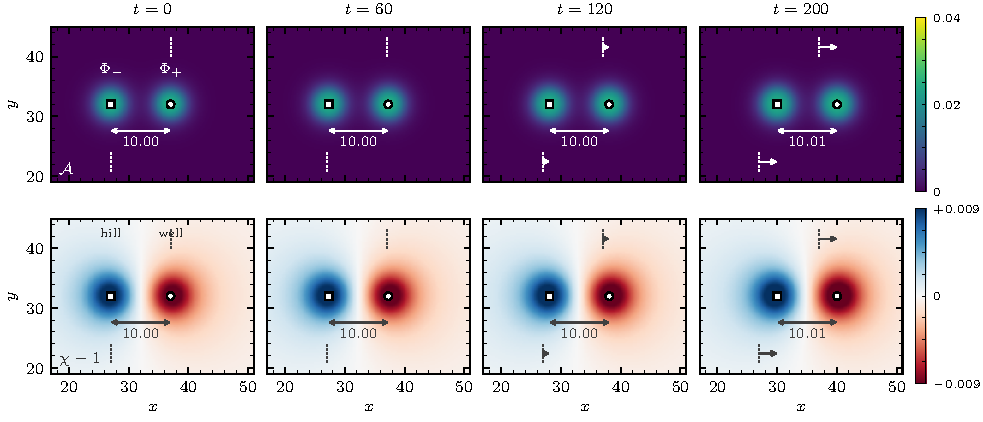
\includegraphics{fig_chase_frames.pdf}
\caption{The runaway in the reference cell (\texttt{PM}, $d_0=12$, $\Delta x=0.25$), $z=0$ plane, at $t=0$, $40$, $50$, $60$. Top: scalar-field activity $\mathcal{A}=\sum_k(\varphi_k^2+\Pi_k^2)^{1/2}$, both sectors. Bottom: $\chi-1$; the phantom star is a hill ($\chi>1$), the canonical star a well ($\chi<1$). Open markers: measured sector barycentres (circle $\Phi_+$, square $\Phi_-$); dashed ticks mark the release positions $x=\pm6$, arrows the displacement since release, and the bracketed number is the measured gap, $12.00\rightarrow11.43\rightarrow11.05\rightarrow10.14$. Both stars move toward $+x$ while the gap slowly closes. Panels are individually colour-scaled.}
\label{fig:frames}
\end{figure*}

\begin{figure*}[t]
\centering
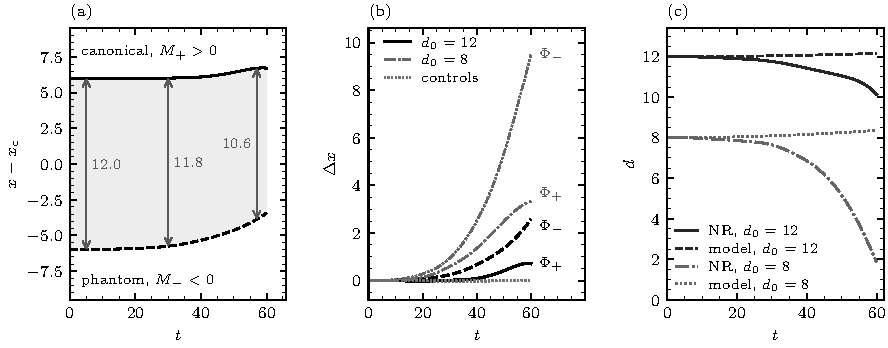
\includegraphics{fig_trajectories.pdf}
\caption{Worldlines and drifts, finest campaign grids only. (a)~The two sector barycentres of the reference cell, released at rest at $x=\pm6$: both move toward $+x$, the phantom (dashed) chasing the canonical star (solid), with the gap measured at $t=5$, $30$ and $57$ ($12.0\rightarrow11.8\rightarrow10.6$). (b)~Sector drifts $\Delta x$: the reference $d_0=12$ cell in black, the contact-contaminated $d_0=8$ cell in gray, and the same-sign controls dotted along the axis; curve ends are labelled by sector. (c)~The gap $d(t)$ for each configuration against its \emph{own} matched point-mass Bondi integration: the model keeps the gap open, the simulations close it, and the discrepancy shrinks with separation (Sec.~\ref{sec:sepscaling}).}
\label{fig:traj}
\end{figure*}

\section{Results}
\label{sec:results}

\subsection{The runaway}
\label{sec:runaway}

Figures~\ref{fig:frames} and \ref{fig:traj} carry the headline. In the reference cell---canonical star released at rest at $x=+6$, phantom at $x=-6$---\emph{both} barycentres move toward $+x$. By $t=60$ the canonical star has moved $+0.71$ and the phantom $+2.57$, so the pair barycentre has drifted $\Delta X = +1.64$ while the gap closed from $12.00$ to $10.14$. The motion is a sustained acceleration from rest, not an impulse: the pair barycentre passes $\Delta X = +0.018$ at $t=15$, $+0.033$ at $t=20$, $+0.131$ at $t=30$ and $+0.380$ at $t=40$.

The barycentre \emph{speeds} (Fig.~\ref{fig:velocity}) say the same thing kinematically. (Speeds, like everything else, are in code units with $c=1$.) In the reference cell the phantom reaches $v_x\approx0.027$ at the clean-window edge $t=30$ and $\approx0.15$ by $t=60$; the canonical star reaches $\approx0.004$ and peaks near $0.047$ at $t\approx52$ before the halo bias of Sec.~\ref{sec:caveats} drags the tracked centroid back. In the contact-contaminated $d_0=8$ cell the same curves run several times higher---phantom $0.107$ at $t=30$, peaking at $0.438$, a genuinely relativistic infall---which is why that cell makes the better picture and the worse measurement.

Two features of the reference run deserve flagging immediately, because both are diagnostic artefacts rather than physics and both are quantified in Sec.~\ref{sec:caveats}. The canonical sector's drift is slightly \emph{negative} between $t\approx3$ and $t\approx25$, worst at $-0.016$ near $t=19$, before turning around: at this separation the phantom's repulsion pushes canonical field toward the $+x$ boundary faster than the star itself moves, and losing the leading edge drags the field-weighted centroid backwards. And the canonical sector's tracked weight falls to $0.39$ of its initial value by $t=60$. Neither affects the phantom sector, which \emph{gains} tracked weight ($1.22\times$ by $t=60$) rather than losing it, and neither can produce a systematic drift of one sign in the pair barycentre---which is why the controls below, not an error model, set the noise floor.

\begin{figure}[t]
\centering
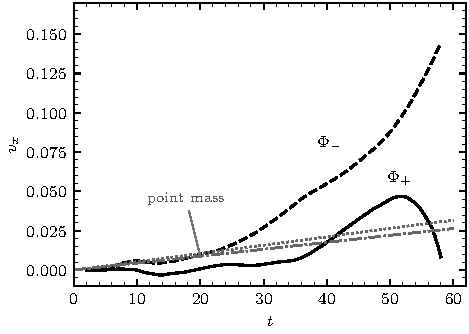
\includegraphics{fig_velocity.pdf}
\caption{Barycentre velocities in the reference cell, in code units ($c=1$): centred differences of the continuously sampled barycentre stream over $\pm2$ time units ($\Phi_+$ solid, $\Phi_-$ dashed), against the matched point-mass model (gray). The phantom passes $v_x=0.027$ at $t=30$ and reaches $\approx0.15$ by $t=60$; the canonical curve turns over near $t\approx52$ as the halo bias of Sec.~\ref{sec:caveats} takes hold, which is a diagnostic effect and not a deceleration.}
\label{fig:velocity}
\end{figure}

\subsection{Only the mixed pair moves}
\label{sec:controls}

The controls are the experiment's null hypothesis, and they are run under numerics identical to the pairs---same code, same gauge, same dissipation, same solve tolerance, same grids. Figure~\ref{fig:controls} collects them.

At $t=60$ the two-canonical pair \texttt{PP} has drifted $+0.036$ and the two-phantom pair \texttt{MM} $+0.012$, against the reference pair's $+1.64$: factors of $46$ and $142$. Both control residuals are smaller than one cell width of the grid they were measured on ($\Delta x=0.25$), and both \emph{shrink} as that grid is refined---\texttt{PP} runs $+0.149$, $+0.080$, $+0.036$ down the ladder and \texttt{MM} $+0.039$, $+0.014$, $+0.012$---which is the signature of a numerical residual, not a physical drift. The single stars, available at the production resolution $\Delta x = 0.5$, drift $+0.061$ and $+0.065$ by $t=40$.

Two honesty notes on this comparison. The same-sign controls sit at $d_0=8$, not at the reference separation, because they were built alongside the original $d_0=8$ series; a closer pair is if anything \emph{more} prone to spurious centroid motion, so using them as the floor is conservative. And against the strong-signal $d_0=8$ mixed cell the same controls come out $179$ and $545$ times smaller---the larger multiples that configuration buys, quoted here only to show that the reference numbers are the cautious ones.

\begin{figure*}[t]
\centering
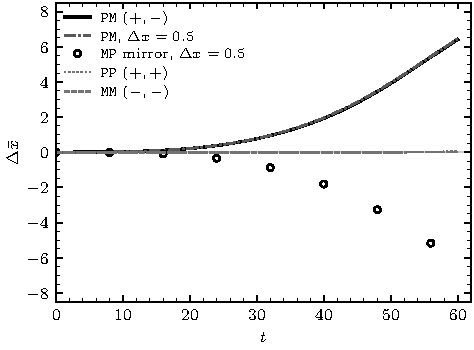
\includegraphics{fig_controls.pdf}
\caption{The four sign assignments under identical numerics. (a)~Pair-barycentre drift at $d_0=8$: the mixed pair \texttt{PM} runs away to $+6.41$, its space-reflected twin \texttt{MP} to $-6.15$ (a $4.7\%$ asymmetry, both at $\Delta x=0.5$), while \texttt{PP} and \texttt{MM} stay on the axis. (b)~The same-sign residuals magnified, at all three resolutions: \texttt{PP} reaches $+0.036$ and \texttt{MM} $+0.012$ at $t=60$---$179$ and $545$ times smaller than the mixed pair, both below one cell width of the finest grid, and both shrinking as the grid is refined.}
\label{fig:controls}
\end{figure*}

\subsection{The mirror control closes the artifact objection}

A drift produced by grid anisotropy, boundary asymmetry, or diagnostic bias would not know which star is which; swapping the sectors in place must reverse the physics but not an artifact. It reverses the physics. Reflected about $x=0$, the mirrored run \texttt{MP} reproduces the reference trajectory of the same numerics to $3.4\%$ in the canonical sector and $5.2\%$ in the phantom sector at $t=60$ (Fig.~\ref{fig:mirror}), and its pair barycentre reaches $-6.15$ against $+6.45$ for the unmirrored run---a $4.7\%$ asymmetry. Both runs of this pair exist only at the production resolution $\Delta x=0.5$, which is why the comparison is made there rather than on the finest grid; that is the correct control anyway, since a mirror test must hold everything except the reflection fixed.

\begin{figure}[t]
\centering
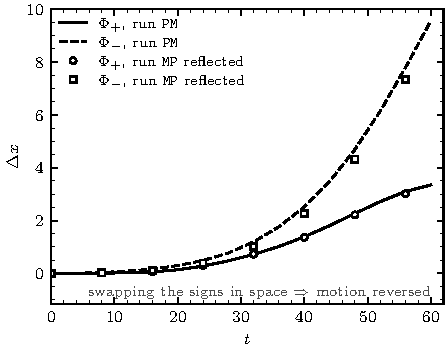
\includegraphics{fig_mirror.pdf}
\caption{The mirror test, sector by sector, at fixed numerics ($\Delta x=0.5$). Lines: run \texttt{PM}. Markers: run \texttt{MP}, in which the two sectors are swapped in space, with its trajectory reflected about $x=0$. Swapping the signs in space reverses the motion, and reproduces its magnitude to a few percent---an artifact of the grid, the boundaries, or the centroid definition would do neither.}
\label{fig:mirror}
\end{figure}

\subsection{Grid convergence}
\label{sec:convergence}

Every configuration in the campaign was run at $\Delta x = 0.50$, $0.33$ and $0.25$ under otherwise identical settings. The logic of the test is the one that applies whenever an effect and its possible artefacts live on the same grid: a physical drift should be insensitive to the grid, and a numerical one should converge away. Figure~\ref{fig:convergence} shows both halves happening at once.

In the reference cell the three resolution curves lie on top of one another for the whole run, ending at $+1.746$, $+1.677$ and $+1.642$---a spread of $6.3\%$ at $t=60$ and $6.6\%$ at $t=30$. The contact-contaminated $d_0=8$ cell is tighter still ($6.4365$, $6.4253$, $6.4065$; $0.5\%$), as is its equal-$|M|$ variant ($0.3\%$), simply because the signal there is larger relative to the same numerical noise. Meanwhile the \texttt{PP} residual falls by a factor of roughly two at each refinement step and \texttt{MM} by a factor of three overall, so that the gap between the physical signal and the numerical floor \emph{widens} monotonically with resolution. That is the convergence statement this paper makes, and it is the one that matters: refinement does not erode the runaway, it isolates it.

At $d_0=16$ the test fails, and we report it as such. The drift there spreads $17\%$ at $t=15$, $41\%$ at $t=30$ and $53\%$ at $t=60$ across the ladder---the signal has fallen to the level where the grid still controls it. Every statement about $d_0=16$ in this paper is therefore a bound, not a measurement.

One caveat must accompany all of this, because the natural next question is what convergence \emph{order} the campaign achieves, and the honest answer is that the campaign cannot report one. A single elliptic solve, performed on its own fixed solver grid, supplies the initial data for all three evolutions of a ladder. Its residual is consequently identical across the ladder, and it dominates the constraint violation from $t\gtrsim1$ onward: the coarse-to-fine ratio of $L_2(\mathcal{H})$ is $1.05\times$ at every sampled time in every mixed-pair ladder (Appendix~\ref{app:constraints}), where a truncation-dominated violation would show a factor of ${\sim}16$. Richardson extrapolation against that floor would measure the solve, not the evolution. We therefore quote the ladder spread as an empirical error bar on every drift---$6.3\%$ on the reference measurement---and defer a formal order to a campaign in which the solve tolerance is refined together with the evolution grid.

\begin{figure*}[t]
\centering
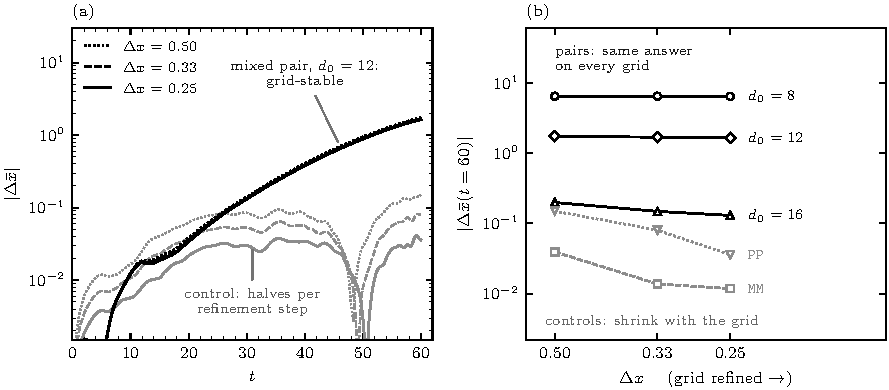
\includegraphics{fig_convergence.pdf}
\caption{The convergence study. (a)~The reference cell's resolution ladder in time (dotted $\Delta x=0.50$, dashed $0.33$, solid $0.25$) against the \texttt{PP} control's ladder: the mixed-pair curves lie on top of one another while the control's residual drift roughly halves at every refinement step. (b)~The same data read as a refinement sequence---$|\Delta \bar{x}|$ at $t=60$ against grid spacing, grid refined to the right---for every family in the campaign. The mixed pairs sit on plateaus (spread $0.5\%$ at $d_0=8$, $6.3\%$ at $d_0=12$) while the same-sign controls fall towards zero. The under-resolved $d_0=16$ family is the exception that proves the test works: its $53\%$ spread is why it is quoted as a bound. No convergence \emph{order} is quotable, because one elliptic solve on a fixed grid feeds all three evolutions of every ladder and floors the constraint violation identically; the spread is the error bar.}
\label{fig:convergence}
\end{figure*}

\subsection{Gravity scales with the source}
\label{sec:scaling}

The strongest quantitative tests compare runs that differ in exactly one quantity. Both are available in the $d_0=8$ family, where \texttt{PM-eq} retunes the phantom to $|M_-|=M_+$ and changes nothing else; the contact contamination of that separation affects both runs identically and largely cancels from the ratios below.

\emph{The push scales with the phantom's active mass.} Between \texttt{PM} and \texttt{PM-eq} the phantom's mass changes by the factor $0.06395/0.07696=0.831$. The canonical star's displacement responds in proportion (Table~\ref{tab:massscaling}): the measured drift ratio is $0.825$ at $t=15$, $0.843$ at $t=20$ and $0.863$ at the window edge $t=30$---within $0.7\%$, $1.5\%$ and $3.9\%$ of the bare mass ratio, and tracking the matched point-mass ratio, which drifts the same way and for the same reason, to better than $3\%$ throughout.

\emph{The fall depends only on the other body.} In the same pair of runs the canonical source is unchanged, and so is the phantom's trajectory: drift ratio $1.022$ at $t=15$, $1.004$ at $t=20$, $1.025$ at $t=30$ and $1.004$ at $t=60$. Two independent solves and evolutions, differing in the phantom's own mass by $17\%$, reproduce its trajectory to $0.4$--$2.6\%$ across the clean window---a physics statement and a reproducibility check at once.

\begin{table}[t]
\caption{Does the push scale with its source? Between runs \texttt{PM-eq} and \texttt{PM} exactly one physical input changes: the phantom's mass magnitude, smaller by the factor $0.06395/0.07696=0.831$. If the canonical star's motion is gravity sourced by the phantom, its drift must shrink by that same factor. ``NR ratio'': the measured canonical-star drift of \texttt{PM-eq} divided by that of \texttt{PM}, both at $\Delta x=0.25$; next to it, the same ratio predicted by the matched point-mass integrations, and the bare mass ratio itself. The last column is the phantom's own drift ratio, which the sign structure requires to be $1$.}
\label{tab:massscaling}
\begin{ruledtabular}
\begin{tabular}{lcccc}
$t$ & NR ratio & point-mass & mass ratio & $\Phi_-$ ratio \\
\hline
$15$ & $\mathbf{0.825}$ & $0.831$ & $0.831$ & $1.022$ \\
$20$ & $\mathbf{0.843}$ & $0.832$ & $0.831$ & $1.004$ \\
$30$ & $0.863$ & $0.834$ & $0.831$ & $1.025$ \\
$40$ & $0.877$ & $0.837$ & $0.831$ & $1.033$ \\
$60$ & $0.881$ & $0.843$ & $0.831$ & $1.004$ \\
\end{tabular}
\end{ruledtabular}
\end{table}

\subsection{Separation dependence}
\label{sec:sepscaling}

The remaining physical knob is the release separation, and it settles what the excess over Newtonian point masses is made of. Fixed-time power-law fits are useless here---the closing gap makes them report exponents between $2$ and $5$, measuring runaway feedback rather than the force law---so each run is compared against its \emph{own} point-mass Bondi integration: two point particles carrying the stars' ADM masses, released at rest at the same separation, each accelerated by the other's active mass. Table~\ref{tab:pointmass} gives the reference cell against that model, and Table~\ref{tab:sepratios} the excess as a function of separation.

The pattern is unambiguous. At $d_0=8$, where the envelopes overlap from $t=0$, the phantom's fall runs $1.4\times$ the point-mass rate at $t=20$ and $5.4\times$ by $t=60$: the phantom sits deep inside the canonical star's near field, where the local pull exceeds the point-mass value $M/d^2$ evaluated at the barycentric separation, and the canonical well deepens further as it re-accretes its shed field ($\chi_{\min}$ falling from $0.98$ to $0.43$). At the reference separation the excess is much smaller---$0.93\times$ at $t=20$, $1.24\times$ at $t=30$---so the measured motion is Newtonian to within $7\%$ early and $24\%$ at the window edge, with the excess growing only as the gap starts to close in earnest. At $d_0=16$ the ratios are $0.87$ and $0.98$, consistent with the point-mass law, though at that separation the drift is not grid-stable and the agreement is only a bound.

\begin{table}[t]
\caption{The reference run against the Newtonian idealization. ``NR'': \texttt{PM} at $d_0=12$, $\Delta x=0.25$, as measured. ``model'': its matched point-mass Bondi integration---two point particles carrying the stars' ADM masses ($+0.0640$ and $-0.0770$), released at rest at $d_0=12$, each accelerated by the \emph{other's} active mass per Sec.~\ref{sec:model}. The canonical column is biased low by the halo (Sec.~\ref{sec:caveats}), which is why the phantom column carries the comparison; the clean window is $t\lesssim30$.}
\label{tab:pointmass}
\begin{ruledtabular}
\begin{tabular}{lcccccc}
& \multicolumn{2}{c}{drift $\Phi_+$} & \multicolumn{2}{c}{drift $\Phi_-$} & \multicolumn{2}{c}{gap} \\
$t$ & NR & model & NR & model & NR & model \\
\hline
$10$ & $+0.00$ & $+0.03$ & $+0.02$ & $+0.02$ & $11.98$ & $12.00$ \\
$20$ & $-0.02$ & $+0.11$ & $+0.08$ & $+0.09$ & $11.90$ & $12.02$ \\
$30$ & $+0.01$ & $+0.24$ & $+0.25$ & $+0.20$ & $11.77$ & $12.04$ \\
$40$ & $+0.09$ & $+0.43$ & $+0.67$ & $+0.35$ & $11.43$ & $12.07$ \\
$60$ & $+0.71$ & $+0.96$ & $+2.57$ & $+0.80$ & $10.14$ & $12.16$ \\
\end{tabular}
\end{ruledtabular}
\end{table}

\begin{table}[t]
\caption{Excess over the point-mass idealization: the ratio of the measured phantom drift to each run's \emph{own} matched point-mass integration, at $\Delta x=0.25$. The excess is an extended-body effect and falls with separation. At $d_0=8$ the stars overlap from $t=0$; at $d_0=16$ the drift is not grid-stable (Sec.~\ref{sec:convergence}) and the entries bound rather than measure.}
\label{tab:sepratios}
\begin{ruledtabular}
\begin{tabular}{lcccc}
$d_0$ & $t=20$ & $t=30$ & $t=40$ & $t=60$ \\
\hline
$8$ (overlapping) & $1.43$ & $2.10$ & $3.14$ & $5.35$ \\
$12$ (reference) & $0.93$ & $1.24$ & $1.88$ & $3.23$ \\
$16$ (bound only) & $0.87$ & $0.98$ & $1.31$ & $1.32$ \\
\end{tabular}
\end{ruledtabular}
\end{table}

\subsection{The phantom sector is the stable one}

Counter to intuition, the phantom star was the best-behaved object in the campaign. Gravity is not its binding agent---the identical scalar self-interaction is---and the reversed sign is the \emph{stabilizing} correction. Shed field around the canonical star is pulled back, deepening the well and feeding perturbations; around the phantom it anti-gravitates and self-dilutes. The extremal conformal factor makes the contrast quantitative across the whole campaign at $\Delta x=0.25$: by $t=60$ the reference cell has reached $\chi_{\min}=0.205$, the $d_0=8$ cell $0.434$, and the merging \texttt{PP} control $0.499$, while the mutually repelling \texttt{MM} control has stayed at $\chi=0.989$ after passing through $1.001$---flat to a part in $10^3$ while its material spreads. The single-star records tell the same story (Table~\ref{tab:stability}): the canonical star's tracked distribution more than doubles in extent over $t=0\rightarrow40$ while the phantom's grows by a seventh.

\begin{table}[t]
\caption{Single-star health, $t=0\rightarrow40$, at the production resolution $\Delta x=0.5$. Extremal $\chi$ is the minimum for the canonical star and the maximum for the phantom; the rms radius includes the radiation bath.}
\label{tab:stability}
\begin{ruledtabular}
\begin{tabular}{lcc}
metric & canonical & phantom \\
\hline
extremal $\chi$ & $0.989\rightarrow0.851$ & $1.000\rightarrow1.001$ \\
rms radius & $5.05\rightarrow12.25$ & $5.43\rightarrow6.25$ \\
peak breathing & $\pm8\%$ & $\pm3\%$ \\
\end{tabular}
\end{ruledtabular}
\end{table}

\section{The gravitational-wave signature}
\label{sec:weyl}

A uniquely relativistic consequence of the runaway is gravitational bremsstrahlung: the exact accelerating-pair metrics are radiative~\cite{bonnor_swami1964,bicak1983}, and negative-mass binaries have recently been proposed as sources of anomalous gravitational-wave signatures with no positive-mass counterpart~\cite{trivedi_loeb2026}. Our runs record the geometry-side diagnostic: the five $\ell=2$ spin-weighted spherical-harmonic amplitudes $r\,\psi_4^{2m}$ of the Weyl scalar $\Psi_4$, summarized by the total amplitude $A_{\ell=2}=[\sum_m|r\,\psi_4^{2m}|^2]^{1/2}$. We take the near zone and the wave zone in turn, because the two answer different questions and only the second requires the larger box.

\subsection{The near-zone signal tracks the source}

On the $L=64$ domain both extraction shells ($R=8$ and $16$) sit inside the massive-field radiation bath, and the amplitude falls steeply between them---$A(R{=}8)$ exceeds $A(R{=}16)$ by $5\times$ at $t=30$ and $10\times$ at $t=60$, far from the $r^{0}$ peeling of a wave-zone signal. What follows is therefore near-zone curvature: the geometry's independent testimony about the source, not a radiated flux.

That testimony is unambiguous (Fig.~\ref{fig:weyl}). The waveform itself resembles no binary signal in the astrophysical catalogue: a monotone, chirpless ramp, the shells rising together with no oscillatory train and no propagating front---the time-domain face of near-zone curvature tracking its source. In the mixed cells, and only there, $A_{\ell=2}$ climbs smoothly and monotonically, ending $122$ times above its early-time floor in the reference cell and $232$ to $481$ times in the louder $d_0=8$ family; the same-sign controls fluctuate at their bath level without any secular ramp (\texttt{PP} stays bounded, while \texttt{MM}'s irregular excursions track its own violent spreading as the mutually repelling pair drives its material apart).

The growth is locked to the runaway kinematics: over $5\le t\le55$ the amplitude correlates with the pair speed $|\dot X|$ at $0.996$, with a single scale factor $\kappa=0.0163$ (Fig.~\ref{fig:weyl}c). This is what the source structure dictates, since the signed quadrupole of a rigidly translating dipole grows with the drift, $Q\sim 2Md\,X(t)$, so the near-zone $\ell=2$ curvature rises with the translation. Three checks tie the signal to the physics rather than to the scalar bath or the grid. The mode pattern is the one an $x$-axisymmetric source imprints on a $z$-axis decomposition: power resides in $m=0,\pm2$, with $m=\pm1$ at $0.54\%$. The spectrum is secular, not oscillatory: $99.7\%$ of the amplitude's spectral power lies below $\omega=0.4$, with fractions of $3.8\times10^{-4}$ at the field frequency $\omega=0.55$ and $7.5\times10^{-6}$ at $2\omega$---the $\ell=2$ curvature is not leakage from the oscillating scalar. And the mirrored run reproduces the reference amplitude history to $4.7\%$, extending the artifact rejection of Sec.~\ref{sec:controls} from the matter sector to the Weyl curvature.

\begin{figure}[t]
\centering
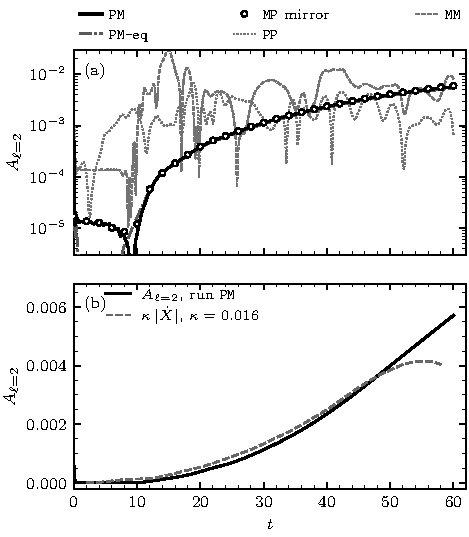
\includegraphics{fig_weyl.pdf}
\caption{The $\ell=2$ Weyl signal at $R=16$, campaign cells at $\Delta x=0.25$ (the mirror overlay exists only at $\Delta x=0.5$). (a)~The raw waveform $r\,\mathrm{Re}\,\psi_4^{2,0}$: in the mixed run a monotone, chirpless ramp; in the same-sign controls a non-secular wander. (b)~Total spin-weighted amplitude $A_{\ell=2}(t)$: the mixed pairs climb by two orders of magnitude ($232\times$ for \texttt{PM}, $350\times$ for the equal-$|M|$ rerun, $481\times$ for the mirror, and $122\times$ in the reference $d_0=12$ cell) while the controls do not. (c)~The amplitude against the rescaled pair speed $\kappa|\dot X|$: correlation $0.996$ over $5\le t\le 55$ with $\kappa\approx0.016$---the near-zone quadrupole rises in lockstep with the runaway, not with the field frequency.}
\label{fig:weyl}
\end{figure}

\subsection{One outgoing wave in the wave zone}
\label{sec:wavezone}

To ask whether any of this is radiation, the shells have to leave the bath, which requires the box rather than the resolution. The \texttt{boxC} series doubles the domain to $L=128$ and places four shells at $r=16$, $24$, $32$ and $40$. One outgoing wave gives the same value of $|r\,\psi_4^{2,0}|$ on every shell when each is read at its own retarded time $u=t-r$; Fig.~\ref{fig:waveconv} performs that test.

There is a clean window, and it is bounded on both sides for understood reasons. Inside $u=10$--$25$ the four shells agree to $1.40\times$, $1.16\times$, $1.10\times$ and $1.33\times$---one wave, propagating outward at the speed of light, on shells spanning a factor of $2.5$ in radius. Before $u\approx10$ they carry the initial-data start-up transient, which has not yet swept past. After $u\approx25$ the expanding canonical envelope reaches them---its rms radius crosses $r=16$ at $t\approx51$---and the shells decouple, spreading to $4.6\times$ by $u=40$. Doubling the box changes the amplitude on the common $r=16$ shell by $0.07$--$0.18\%$ across that window, so the signal is not a boundary reflection: it is box-independent to two parts in a thousand.

What this does \emph{not} settle is the energy budget---whether the net gravitational-wave energy radiated by a mixed pair is positive, negative, or cancels between the sectors. That needs the odd-$\ell$ modes, whose interference with $\ell=2$ carries the momentum-flux beaming along the runaway axis, together with ADM surface integrals at the outer boundary and a sponge layer to extend the window past the arrival of the matter. That extraction---benchmarked against the Bonnor--Swaminarayan acceleration parameter~\cite{bonnor_swami1964}---is the geometry-side program for the follow-up campaign.

\begin{figure}[t]
\centering
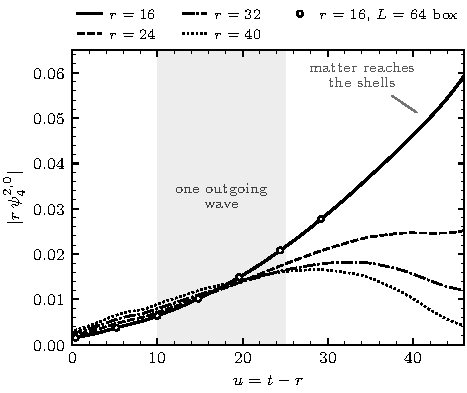
\includegraphics{fig_waveconv.pdf}
\caption{One outgoing wave, from the double-size box ($L=128$, $\Delta x=0.5$). $|r\,\psi_4^{2,0}|$ on the four wave-zone shells $r=16$, $24$, $32$, $40$, each plotted against its own retarded time $u=t-r$. Inside the shaded window $u=10$--$25$ the four shells agree to $1.10$--$1.40\times$; before it they carry the start-up transient, after it the expanding matter reaches them. Open circles: the half-size $L=64$ box at $r=16$, differing by $0.07$--$0.18\%$---the amplitude is box-independent.}
\label{fig:waveconv}
\end{figure}

\subsection{Is there dipole radiation?}

For binaries whose members carry different ratios of gravitational charge to inertial mass, the leading anomalous channel is dipolar, and binary-pulsar bounds on that channel exclude opposite-gravitational-charge pairs by orders of magnitude---but, as Ref.~\cite{trivedi_loeb2026} emphasizes, only for \emph{non-universal} coupling. The bicomplex model closes the channel structurally. The source of gravity is the signed stress tensor, conserved on shell (Sec.~\ref{sec:model}); the rate of change of the signed mass dipole is therefore the conserved signed momentum---near zero for pairs released at rest---so mass-dipole radiation is forbidden at leading order for exactly the reason it is forbidden in ordinary general relativity. At the point-mass level the cancellation is the reciprocity $M_+a_+=|M_-|\,a_-=M_+|M_-|/d^2$, which holds for unequal magnitudes too. Kinematics agrees from the other side: $\Psi_4$ carries spin weight $-2$, so its multipole expansion begins at $\ell=2$---there is no $\ell=1$ mode to populate. The anomalous gravitational-wave channel of a Bondi dipole is therefore not dipolar emission but the signature Fig.~\ref{fig:weyl} shows in embryo: the ever-growing quadrupole of a linearly accelerating, near-zero-total-mass system---bremsstrahlung without inspiral, secular where every astrophysical binary chirps.

One structural feature of the budget does not wait on the measurement: it has no floor. The pair begins with essentially no mass to spend---$M_++M_-=-0.013$ in the reference configuration and zero to five digits in \texttt{PM-eq}---while the Bondi mass-loss formula is purely geometric, the news-squared flux being positive-definite irrespective of what sources the field. A radiating isolated system therefore loses mass monotonically, and this one does so starting from zero. Nothing arrests the descent, because the bound that would arrest it is the positive-mass theorem, whose hypothesis this matter violates by construction (Sec.~\ref{sec:intro}): there is no minimum-energy configuration for the pair to relax into, hence no terminus. The runaway is thus secular in its energetics as much as in its kinematics---a radiating system with no ground state, the classical face of the graviton-mediated vacuum instability that already bars this matter quantum-mechanically~\cite{carroll2003,cline2004}, and part of why we present the model as a classical probe. It also sharpens the purpose of the wave-zone campaign: the question is not only how large the flux is, but whether its sign is the positive one this argument presumes.

It is tempting to read the gap closure of Sec.~\ref{sec:sepscaling} as reinstating mass-dipole emission---with $|M_-|=M_+$ the signed dipole collapses to $D=M_+(x_+-x_-)=M_+d$, static for the textbook constant-gap runaway and plainly not static here---but the inference fails on both sides. Structurally, a spin-weight-$-2$ field has no $\ell=1$ harmonic to populate whatever $\ddot D$ does. Dynamically, $\dot D$ is a momentum rather than a source, and which momentum matters: for the whole system it is the ADM momentum, conserved and zero for data released at rest, so the total $\ddot D$ vanishes identically; for the matter alone it is the volume-integrated sector momentum, which is \emph{not} separately conserved. The stream measures exactly that distinction. In \texttt{PM-eq}, where $M_++M_-=0$ reduces the matter dipole rate to $M_+\dot d$, the measured signed momentum tracks $M_+\dot d$ to $6$--$14\%$ across the clean window---field volume integrals and independent core tracking agreeing on one number. So the matter dipole does accelerate; the compensating momentum resides in the gravitational field, which is precisely why closing the balance requires surface integrals rather than volume ones. What the closing gap genuinely adds is a second time dependence in the \emph{quadrupole}, superposed on the linear acceleration that dominates Fig.~\ref{fig:weyl}.

\section{Caveats, and their measured scope}
\label{sec:caveats}

\emph{The barycentre includes the halo.} Equation~\eqref{eq:barycentre} integrates core plus shed radiation over the whole domain. In the reference cell the canonical sector's tracked weight holds to $1.2\%$ through $t=20$ and $4.2\%$ through $t=30$, then falls away to $0.39$ of its initial value by $t=60$ as field leaves the accounting region; the phantom's weight instead grows steadily, by $6\%$ at $t=20$ and $22\%$ by $t=60$. The clean quantitative window is therefore $t\lesssim30$---exactly where the mass-scaling and reproducibility tests are strongest---and late-time canonical drifts are upper bounds on core displacement. The qualitative result holds across the whole run, and the pair barycentre, whose controls are exactly zero by symmetry, is the quantity least exposed to this.

\emph{The canonical centroid is biased low.} Losing the leading edge of a distribution drags its centroid backwards, so canonical drifts are underestimates everywhere, worst where the true displacement is small---wide gaps and early times. The reference run shows it directly: the canonical sector reads slightly negative between $t\approx12$ and $t\approx25$ before turning around, and at $d_0=16$ it never recovers, ending at $-0.33$. The phantom sector, which gains tracked weight rather than losing it, is the trustworthy one, and Sec.~\ref{sec:sepscaling} uses it; the mass-scaling ratio compares equal-separation runs, so the bias largely cancels there. A core-weighted centroid immune to the halo is built for the follow-up.

\emph{Resolution, and what the ladder does and does not establish.} Every cell was run at three grid spacings, and the mixed-pair drift is stable across them---$6.3\%$ in the reference cell, $0.5\%$ at $d_0=8$---while the control residuals converge away (Sec.~\ref{sec:convergence}). That establishes the effect is not a grid artefact. It does not establish a convergence order, because one elliptic solve on a fixed grid feeds all three evolutions of every ladder and floors the constraint violation identically; refining the solve alongside the grid is the outstanding piece of work here. And the test has a floor of its own: at $d_0=16$ it fails, which is why that separation is quoted as a bound throughout.

\emph{The radiation bath cannot leave.} Massive-field radiation reflects from massless-wave (Sommerfeld) boundaries and washes back over the stars; this caps the mixed runs at $t=60$. Doubling the box (Sec.~\ref{sec:wavezone}) shows the extracted amplitude is insensitive to the boundary at the level of $0.2\%$ inside the clean window, but does not remove the bath itself. A sponge layer is the fix, and is what a constant-gap test at $t\gg60$ requires.

\emph{Gauge.} The barycentres of Eq.~\eqref{eq:barycentre} are coordinate quantities in a dynamical gauge. The mirror test (Sec.~\ref{sec:controls}) and the Weyl correlation (Sec.~\ref{sec:weyl}) are the two checks that do not depend on that choice, and both agree with the coordinate measurement.

\section{Discussion and conclusion}
\label{sec:discussion}

\emph{What is established.} We posed Bondi's positive--negative mass pair as a full initial-value problem, and it behaved exactly as he argued in 1957. The main results, restated:
\begin{itemize}
\item[(1)] \emph{The runaway is real in full general relativity.} Released at rest, the mixed pair---and only the mixed pair---self-accelerates, the phantom chasing the canonical star. In the reference configuration the pair barycentre drifts $+1.64$ by $t=60$, $46$ times the two-canonical control and $142$ times the two-phantom one, and reverses under mirror reflection to $4.7\%$. The geometry testifies independently of the matter diagnostics: the $\ell=2$ Weyl amplitude rises in lockstep with the runaway speed (correlation $0.996$) and mirrors with the configuration (Sec.~\ref{sec:weyl}).
\item[(2)] \emph{The measurement survives grid refinement.} Across $\Delta x = 0.50$, $0.33$ and $0.25$ the reference drift is stable to $6.3\%$ while the control residuals fall by factors of $3$--$4$, so refinement widens the separation between signal and floor rather than eroding it (Sec.~\ref{sec:convergence}). No convergence order is quoted, and the reason---a shared elliptic-solve floor---is stated rather than hidden.
\item[(3)] \emph{The effect responds to its source the way gravity must.} The push on the canonical star scales with the phantom's active mass to $0.7$--$3.9\%$ across the clean window; the phantom's fall is set by the canonical star alone, reproducing across independent solves to $0.4$--$2.6\%$; and the excess over the matched point-mass prediction falls monotonically with separation, from $2.1\times$ at $d_0=8$ to $1.24\times$ at the reference separation and $0.98\times$ at $d_0=16$, all at $t=30$.
\item[(4)] \emph{Momentum bookkeeping balances as the point-mass kinematics demands.} The volume-integrated signed momentum $P^{\rm signed}_x(t)=\int\bigl(S_x[\Phi_+]-S_x[\Phi_-]\bigr)\,d^3x$ shows the two sectors' momenta---each growing to $(5$--$7)\times10^{-3}$ by $t=30$---cancelling to a residual $2.6$--$4.0\times$ smaller. That residual is not truncation error: it reproduces the point-mass sum $M_+v_+ + M_-v_-$, built from independently tracked core velocities and the dressed ADM masses, to about $10\%$ over $20\le t\le30$. A pair of net mass $M_++M_-\simeq-0.013$ \emph{must} carry $P=M_{\rm net}\,v$; Forward's near-zero total is the equal-$|M|$ idealization. The equal-$|M|$ pair removes that term yet keeps a comparable residual, $M_+(v_+-v_-)$, because its gap slowly closes---a finite-size effect outside Bondi's constant-gap picture at that separation. What remains expectation rather than measurement is the field-side closure---matter plus gravitational-field momentum summing to zero---which needs the ADM surface integral on an enlarged domain; small momentum-\emph{constraint} norms (Appendix~\ref{app:constraints}) remain a distinct statement.
\item[(5)] \emph{A stable star with negative ADM mass exists} as constraint-satisfying, asymptotically flat initial data and survives dynamical evolution---to our knowledge a first in this setting (static phantom-field stars~\cite{dzhunushaliev2014} and de Sitter bubbles~\cite{mbarek2014} were known), and possibly the most reusable artifact of the campaign, since the phantom star proved the best-behaved object in it.
\end{itemize}

\emph{What is not established.} A \emph{constant-gap} runaway---the textbook picture of the pair accelerating forever at fixed separation---requires point-like separation, and we do not reach it. At $d_0=8$ the stars overlap and close to near-contact by $t=60$; at the reference separation the closure is far milder ($12.00\rightarrow10.14$) but still present; at $d_0=16$ the gap is nearly constant, and there the drift is no longer grid-stable. The clean test needs wide separation \emph{and} a longer window, which means a sponge layer and a larger domain rather than a finer grid.

Raising $\omega$ helps only partially, and not in the way one might expect. The dressed family is non-monotonic in radius: $R_{90}$ of the canonical star falls from $7.57$ at $\omega=0.550$ to a minimum of $5.11$ at $\omega\simeq0.80$ and then inflates again in the thick-wall limit, while $R_{99}$---which includes the exponential tail---turns over much earlier, at $\omega\simeq0.62$. So there is a bounded $32\%$ reduction in core radius available, and the sector mass asymmetry does improve markedly over the same interval ($20.3\%\rightarrow4.3\%$ in $|M_-|/|M_+|-1$; Fig.~\ref{fig:family}). But the stars do not become more \emph{compact}: $2|M|/R_{99}$ decreases monotonically across the whole family, by a factor $6.4$ between $\omega=0.550$ and $0.80$ (a factor ${\sim}15$ over $0.53\le\omega\le0.90$), because the ADM mass falls faster than the radius. Higher $\omega$ therefore buys a better separation-to-size ratio and a more symmetric pair at the cost of a weaker signal, and cannot substitute for the larger domain.

Every mixed run was stopped before contact; what a canonical--phantom collision produces---including whether a horizon forms---is untouched, though Mann's negative-mass black holes~\cite{mann1997} make the question sharper than it looks. And nothing here bears on whether NEC-violating matter exists. In that connection the contrast with Nojiri and Odintsov~\cite{nojiri2026} is worth drawing: they find that a positive--negative pair \emph{can} bind, in a setting with a cosmological fluid and a negative cosmological constant supplying the background. Our pair is asymptotically flat and isolated, with nothing to bind against, and it runs away---consistent with both results, and a reminder that the fate of a Bondi dipole is a statement about its environment as much as about its signs.

\emph{Next steps.} A core-weighted centroid immune to the halo, and a solve tolerance refined together with the evolution grid so that a convergence order becomes quotable, are the two diagnostic upgrades. A sponge layer unlocks $t\gg60$ and with it the constant-gap test at $d_0=16$, where the present campaign can only set a bound. Wave-zone extraction on the enlarged domain---with the odd-$\ell$ modes that carry the momentum-flux beaming, ADM mass and momentum surface integrals at the outer boundary, and the Bonnor--Swaminarayan acceleration benchmark~\cite{bonnor_swami1964}---moves the proof from the matter to the geometry and settles the one question Sec.~\ref{sec:weyl} cannot: the sign and budget of the energy this runaway radiates. The contact end state follows.

\section*{Reproducibility}

All time series, star tables, parameter files, code patches, analysis scripts, and the campaign journal behind every number and figure are packed, with machine paths scrubbed, in the repository's results tree (\texttt{results/bondi-dipole-runaway/}); the figures regenerate from that pack by a single script, which also prints every number quoted in the captions and text. Every run lives in \texttt{campaign/}, one directory per cell. The convergence campaign is named \texttt{convA\_<config>\_n<N>} for the $L=64$ series and \texttt{boxC\_<config>\_L128\_n256} for the double box; the reference cell of this paper is \texttt{convA\_pm\_sep12\_n256}. Four earlier production runs at $\Delta x=0.5$ sit alongside them under unprefixed names---\texttt{pair\_pm}, \texttt{pair\_mp\_mirror}, \texttt{single\_p}, \texttt{single\_m}, together with the \texttt{*\_v2} cells carrying the sector-momentum streams. They are used only for the mirror test, the single-star controls, and the momentum bookkeeping, where the convergence campaign has no twin, and their resolution is stated wherever they appear. The star ODE solver of Sec.~\ref{sec:initialdata} and the $M(\omega)$ scan behind Fig.~\ref{fig:family} are \texttt{analysis/star\_family\_scan.py} and the \texttt{boson\_star\_ode} module it drives. Initial data: \texttt{GRTresna}~\cite{grtresna}; evolution: \texttt{GRTeclyn}~\cite{grteclyn}, the AMReX-based~\cite{amrex} GPU port of \texttt{GRChombo}~\cite{grchombo}.

\begin{acknowledgments}
This work was supported by Gravity Frontiers
(\url{https://www.gravityfrontiers.org/en}), which funded the underlying
research and the development of the numerical-simulation software. The author
extends sincere gratitude to Ilya Nachevsky for generously providing the
high-performance computing resources essential to this work, and acknowledges
the GRTL Collaboration for \texttt{GRChombo}, \texttt{GRTresna}, and
\texttt{GRTeclyn}.
\end{acknowledgments}

\appendix

\section{Constraint behaviour}
\label{app:constraints}

\emph{Initial data.} \texttt{GRTresna}'s nonlinear iteration contracts monotonically on every cell of the campaign. The mixed-pair solves converge in seven iterations from $100\%$ to $0.083\%$ (Hamiltonian) and $0.075\%$ (momentum); the two-canonical cells, whose Hamiltonian residual starts already satisfied, need four and exit below $0.004\%$ and $0.049\%$. The worst cell in the campaign exits at $0.094\%/0.079\%$---the gate quoted in Table~\ref{tab:matrix}, in the solver's own grid and normalization.

\emph{Evolution.} The constraints are re-evaluated on the evolution grid every $\Delta t=0.5$ and reduced to composite norms over the domain (outermost four cells excluded so boundary violation is not misread as interior error). Figure~\ref{fig:constraints} shows the record for the reference cell's full ladder, in absolute code units: over an overwhelmingly vacuum domain a global \emph{relative} normalization is dominated by near-zero denominators, so the yardstick is the controls run under identical numerics.

Four features carry the message. The birth transient: re-evaluating with fourth-order stencils after the analytic matter reconstruction (Sec.~\ref{sec:initialdata}) gives $L_2(\mathcal{H})=2.9\times10^{-3}$ at $t=0$ on the finest grid, which relaxes within $t\lesssim1$ to $1.0\times10^{-4}$---the truncation floor---before any secular growth begins. Secular growth: $L_2(\mathcal{H})$ reaches $1.2\times10^{-3}$ at $t=15$, $2.8\times10^{-3}$ at the window edge $t=30$ and $7.7\times10^{-3}$ at $t=60$, with $L_\infty(\mathcal{H})$ at $5.5\times10^{-2}$ and $1.5$, concentrated in the deepening canonical well as the pair evolves and the trapped bath washes back (Sec.~\ref{sec:caveats}); $L_2(\mathcal{M})$ stays below $3.4\times10^{-4}$ through $t=45$ before rising to $1.4\times10^{-3}$ at $t=60$. This growth is the quantitative face of the $t\lesssim30$ window. Comparison with the controls: through that window the mixed run's violation is within a factor $1.8$ of the non-drifting same-sign controls ($2.8\times10^{-3}$ against $1.6\times10^{-3}$ for \texttt{PP} and $2.1\times10^{-3}$ for \texttt{MM} at $t=30$) while the drifts differ by $46$ to $142$ times---the drift correlates with the sign structure, not the constraint error.

And the ladder itself, which is the point of Sec.~\ref{sec:convergence}'s caveat. Refining the grid does \emph{not} reduce the violation: the coarse-to-fine ratio of $L_2(\mathcal{H})$ is $1.04$--$1.06\times$ at $t=15$, $30$, $45$ and $60$ in every mixed-pair ladder, and $0.92$--$1.00\times$ in $L_\infty$. A truncation-dominated violation would fall by a factor of ${\sim}16$ between $\Delta x=0.50$ and $0.25$ at fourth order. It does not, because all three evolutions of a ladder inherit the same initial data from one elliptic solve performed on one fixed solver grid; that residual sets the floor and the evolution grid never gets below it. (At $t=0$ the ratio is $0.31$--$0.37\times$, i.e.\ the violation is nominally \emph{larger} on finer grids, which is the same statement seen at the moment of re-evaluation: a fixed interpolation error resolved by sharper stencils.) This is why the campaign quotes ladder spread as an error bar and no convergence order, and why refining the solve tolerance alongside the grid is the first item of follow-up work.

\begin{figure}[!tb]
\centering
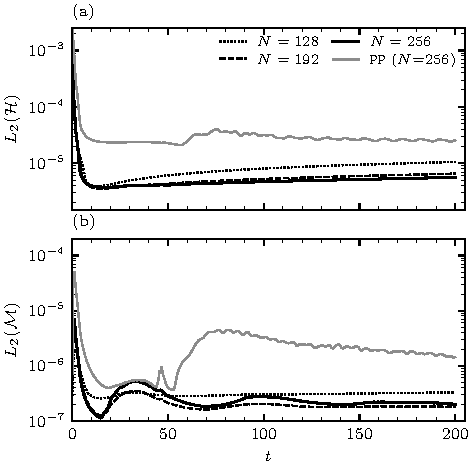
\includegraphics{fig_constraints.pdf}
\caption{Constraint monitoring for the reference cell's resolution ladder (dotted $\Delta x=0.50$, dashed $0.33$, solid $0.25$), against the same-sign controls under identical numerics. (a)~Hamiltonian constraint $\mathcal{H}$: composite $L_2$ norms, plus the finest grid's $L_\infty$. The three ladder curves coincide---the elliptic-solve floor discussed in the text. (b)~Momentum constraint $\mathcal{M}$, $L_2$.}
\label{fig:constraints}
\end{figure}

\FloatBarrier

\begin{thebibliography}{99}

\bibitem{bondi1957}
H.~Bondi,
\newblock ``Negative mass in general relativity,''
\newblock Rev.\ Mod.\ Phys.\ \textbf{29}, 423 (1957).

\bibitem{bonnor_swami1964}
W.~B.~Bonnor and N.~S.~Swaminarayan,
\newblock ``An exact solution for uniformly accelerated particles in general relativity,''
\newblock Z.\ Phys.\ \textbf{177}, 240 (1964).

\bibitem{bicak1983}
J.~Bi\v{c}\'ak, C.~Hoenselaers, and B.~G.~Schmidt,
\newblock ``The solutions of the Einstein equations for uniformly accelerated particles without nodal singularities,''
\newblock Proc.\ R.\ Soc.\ London A \textbf{390}, 397 (1983).

\bibitem{bonnor1989}
W.~B.~Bonnor,
\newblock ``Negative mass in general relativity,''
\newblock Gen.\ Relativ.\ Gravit.\ \textbf{21}, 1143 (1989).

\bibitem{forward1990}
R.~L.~Forward,
\newblock ``Negative matter propulsion,''
\newblock J.\ Propulsion Power \textbf{6}, 28 (1990).

\bibitem{hoffmann1966}
B.~Hoffmann,
\newblock ``Negative mass and the quasars,''
\newblock in \emph{Perspectives in Geometry and Relativity}, edited by B.~Hoffmann (Indiana University Press, Bloomington, 1966), p.~176.

\bibitem{martins1980}
R.~de~A.~Martins,
\newblock ``Causal paradoxes implied by the hypothetical coexistence of positive- and negative-mass matter,''
\newblock Lett.\ Nuovo Cimento \textbf{28}, 265 (1980).

\bibitem{caldwell2002}
R.~R.~Caldwell,
\newblock ``A phantom menace? Cosmological consequences of a dark energy component with super-negative equation of state,''
\newblock Phys.\ Lett.\ B \textbf{545}, 23 (2002).

\bibitem{morris_thorne1988}
M.~S.~Morris and K.~S.~Thorne,
\newblock ``Wormholes in spacetime and their use for interstellar travel: A tool for teaching general relativity,''
\newblock Am.\ J.\ Phys.\ \textbf{56}, 395 (1988).

\bibitem{alcubierre1994}
M.~Alcubierre,
\newblock ``The warp drive: hyper-fast travel within general relativity,''
\newblock Class.\ Quantum Grav.\ \textbf{11}, L73 (1994).

\bibitem{mann1997}
R.~B.~Mann,
\newblock ``Black holes of negative mass,''
\newblock Class.\ Quantum Grav.\ \textbf{14}, 2927 (1997), arXiv:gr-qc/9705007.

\bibitem{nojiri2026}
S.~Nojiri and S.~D.~Odintsov,
\newblock ``May negative mass objects exist in the sky?,''
\newblock arXiv:2602.15058 [gr-qc] (2026).

\bibitem{gleiser2006}
R.~J.~Gleiser and G.~Dotti,
\newblock ``Instability of the negative mass Schwarzschild naked singularity,''
\newblock Class.\ Quantum Grav.\ \textbf{23}, 5063 (2006).

\bibitem{shinkai2002}
H.~Shinkai and S.~A.~Hayward,
\newblock ``Fate of the first traversible wormhole: Black-hole collapse or inflationary expansion,''
\newblock Phys.\ Rev.\ D \textbf{66}, 044005 (2002).

\bibitem{friedberg1976}
R.~Friedberg, T.~D.~Lee, and A.~Sirlin,
\newblock ``Class of scalar-field soliton solutions in three space dimensions,''
\newblock Phys.\ Rev.\ D \textbf{13}, 2739 (1976).

\bibitem{coleman1985}
S.~Coleman,
\newblock ``Q-balls,''
\newblock Nucl.\ Phys.\ B \textbf{262}, 263 (1985).

\bibitem{friedberg1987}
R.~Friedberg, T.~D.~Lee, and Y.~Pang,
\newblock ``Mini-soliton stars,''
\newblock Phys.\ Rev.\ D \textbf{35}, 3658 (1987).

\bibitem{kaup1968}
D.~J.~Kaup,
\newblock ``Klein--Gordon geon,''
\newblock Phys.\ Rev.\ \textbf{172}, 1331 (1968).

\bibitem{ruffini1969}
R.~Ruffini and S.~Bonazzola,
\newblock ``Systems of self-gravitating particles in general relativity and the concept of an equation of state,''
\newblock Phys.\ Rev.\ \textbf{187}, 1767 (1969).

\bibitem{liebling2023}
S.~L.~Liebling and C.~Palenzuela,
\newblock ``Dynamical boson stars,''
\newblock Living Rev.\ Relativ.\ \textbf{26}, 1 (2023).

\bibitem{alic2012}
D.~Alic, C.~Bona-Casas, C.~Bona, L.~Rezzolla, and C.~Palenzuela,
\newblock ``Conformal and covariant formulation of the Z4 system with constraint-violating modes,''
\newblock Phys.\ Rev.\ D \textbf{85}, 064040 (2012).

\bibitem{grchombo}
T.~Andrade \emph{et al.},
\newblock ``GRChombo: an adaptable numerical relativity code for fundamental physics,''
\newblock J.\ Open Source Softw.\ \textbf{6}, 3703 (2021).

\bibitem{grteclyn}
GRTL Collaboration,
\newblock \texttt{GRTeclyn},
\newblock \url{https://github.com/GRTLCollaboration/GRTeclyn}.

\bibitem{grtresna}
J.~C.~Aurrekoetxea, S.~E.~Brady, \emph{et al.},
\newblock ``GRTresna: an open-source code to solve the initial data constraints in numerical relativity,''
\newblock arXiv:2501.13046 [gr-qc] (2025).

\bibitem{amrex}
W.~Zhang \emph{et al.},
\newblock ``AMReX: a framework for block-structured adaptive mesh refinement,''
\newblock J.\ Open Source Softw.\ \textbf{4}, 1370 (2019).

\bibitem{schoen_yau1979}
R.~Schoen and S.-T.~Yau,
\newblock ``On the proof of the positive mass conjecture in general relativity,''
\newblock Commun.\ Math.\ Phys.\ \textbf{65}, 45 (1979).

\bibitem{witten1981}
E.~Witten,
\newblock ``A new proof of the positive energy theorem,''
\newblock Commun.\ Math.\ Phys.\ \textbf{80}, 381 (1981).

\bibitem{mbarek2014}
S.~Mbarek and M.~B.~Paranjape,
\newblock ``Negative mass bubbles in de Sitter spacetime,''
\newblock Phys.\ Rev.\ D \textbf{90}, 101502(R) (2014).

\bibitem{gonzalez2009}
J.~A.~Gonz\'alez, F.~S.~Guzm\'an, and O.~Sarbach,
\newblock ``Instability of wormholes supported by a ghost scalar field. II. Nonlinear evolution,''
\newblock Class.\ Quantum Grav.\ \textbf{26}, 015011 (2009); see also \textbf{26}, 015010 (2009).

\bibitem{dzhunushaliev2014}
V.~Dzhunushaliev, V.~Folomeev, C.~Hoffmann, B.~Kleihaus, and J.~Kunz,
\newblock ``Boson stars with nontrivial topology,''
\newblock Phys.\ Rev.\ D \textbf{90}, 124038 (2014).

\bibitem{carroll2003}
S.~M.~Carroll, M.~Hoffman, and M.~Trodden,
\newblock ``Can the dark energy equation-of-state parameter $w$ be less than $-1$?,''
\newblock Phys.\ Rev.\ D \textbf{68}, 023509 (2003).

\bibitem{cline2004}
J.~M.~Cline, S.~Jeon, and G.~D.~Moore,
\newblock ``The phantom menaced: constraints on low-energy effective ghosts,''
\newblock Phys.\ Rev.\ D \textbf{70}, 043543 (2004).

\bibitem{helfer2022}
T.~Helfer, U.~Sperhake, R.~Croft, M.~Radia, B.-X.~Ge, and E.~A.~Lim,
\newblock ``Malaise and remedy of binary boson-star initial data,''
\newblock Class.\ Quantum Grav.\ \textbf{39}, 074001 (2022).

\bibitem{cttk}
J.~C.~Aurrekoetxea, K.~Clough, and E.~A.~Lim,
\newblock ``CTTK: a new method to solve the initial data constraints in numerical relativity,''
\newblock Class.\ Quantum Grav.\ \textbf{40}, 075003 (2023).

\bibitem{bona1995}
C.~Bona, J.~Mass\'o, E.~Seidel, and J.~Stela,
\newblock ``New formalism for numerical relativity,''
\newblock Phys.\ Rev.\ Lett.\ \textbf{75}, 600 (1995).

\bibitem{campanelli2006}
M.~Campanelli, C.~O.~Lousto, P.~Marronetti, and Y.~Zlochower,
\newblock ``Accurate evolutions of orbiting black-hole binaries without excision,''
\newblock Phys.\ Rev.\ Lett.\ \textbf{96}, 111101 (2006).

\bibitem{baker2006}
J.~G.~Baker, J.~Centrella, D.-I.~Choi, M.~Koppitz, and J.~van~Meter,
\newblock ``Gravitational-wave extraction from an inspiraling configuration of merging black holes,''
\newblock Phys.\ Rev.\ Lett.\ \textbf{96}, 111102 (2006).

\bibitem{trivedi_loeb2026}
O.~Trivedi and A.~Loeb,
\newblock ``Unique gravitational-wave signals from negative-mass binaries,''
\newblock arXiv:2605.10976 [gr-qc] (2026).

\bibitem{shirokov2026}
N.~M.~Shirokov,
\newblock ``Wormhole dynamics: nonlinear collapse and gravitational-wave emission,''
\newblock arXiv:2604.00071 [gr-qc] (2026).

\end{thebibliography}

\end{document}
